\chapter{Preventivo}\label{Preventivo}

In questa sezione il gruppo \textit{Jawa Druids} descrive come userà le risorse a sua disposizione. Per identificarli nelle tabelle, i ruoli vengono indicati con le seguenti sigle:
\begin{itemize}
	\item \textbf{Re}: \textit{Responsabile};
	\item \textbf{Am}: \textit{Amministratore};
	\item \textbf{An}: \textit{Analista};
	\item \textbf{Pt}: \textit{Progettista};
	\item \textbf{Pr}: \textit{Programmatore};
	\item \textbf{Ve}: \textit{Verificatore}.
\end{itemize}
\clearpage
\section{Fase di Analisi}\label{PreventivoFaseDiAnalisi}

\subsection{Prospetto orario}\label{PreventivoFaseDiAnalisiProspettoOrario}
In questa fase la distribuzione oraria è la seguente:
\quad
\def\tabularxcolumn#1{m{#1}}
{\rowcolors{2}{RawSienna!90!RawSienna!20}{RawSienna!70!RawSienna!40}

	\begin{center}
		\renewcommand{\arraystretch}{1.4}
		\begin{tabularx}{\textwidth}{|X|c|c|c|c|c|c|c|}
			\hline
			\rowcolor{airforceblue}
			\textbf{Nominativo} & \textbf{Re} & \textbf{Am} & \textbf{An} & \textbf{Pt} & \textbf{Pr} & \textbf{Ve} & \textbf{Totale ore}\\
			\hline
			\textit{Andrea Dorigo} & 10 & 7 & 3 & 0 & 0 & 5 & 25\\
			\hline
			\textit{Margherita Mitillo} & 8 & 3 & 13 & 0 & 0 & 1 & 25\\
			\hline
			\textit{Igli Mezini} & 3 & 6 & 8 & 0 & 0 & 8 & 25\\
			\hline
			\textit{Andrea Cecchin} & 5 & 9 & 9 & 0 & 0 & 2 & 25\\
			\hline
			\textit{Emma Roveroni} & 2 & 5 & 7 & 0 & 0 & 11 & 25\\
			\hline
			\textit{Alfredo Graziano} & 0 & 10 & 9 & 0 & 0 & 6 & 25\\
			\hline
			\textit{Mattia Cocco} & 1 & 9 & 8 & 0 & 0 & 7 & 25\\
			\hline
			Totale ore ruolo & 26 & 42 & 49 & 0 & 0 & 33 & 150\\
			\hline
		\end{tabularx}
	\captionof{table}{\textbf{distribuzione delle ore durante l'Analisi}}
	\end{center}

Il seguente istogramma riassume i dati ottenuti:
\begin{figure}[!h]
	\begin{center}
		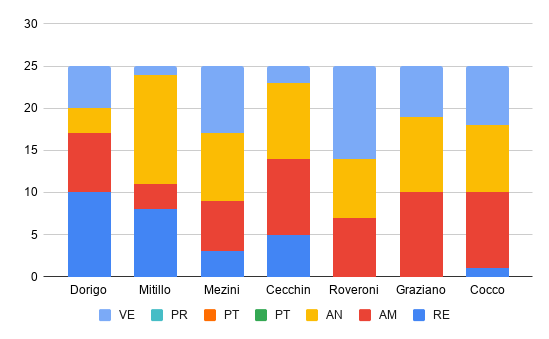
\includegraphics[width=0.7\linewidth]{../immagini/pdp/istogramma_analisi.png}
		\caption{Istogramma della ripartizione oraria durante la Analisi}
	\end{center}
\end{figure}
\clearpage
\subsection{Prospetto economico}\label{PreventivoFaseDiAnalisiProspettoEconomico}
\quad
\def\tabularxcolumn#1{m{#1}}
{\rowcolors{2}{RawSienna!90!RawSienna!20}{RawSienna!70!RawSienna!40}
	\begin{center}
		\renewcommand{\arraystretch}{1.4}
		\begin{tabularx}{7cm}{|X|c|c|}
			\hline
			\rowcolor{airforceblue}
			\textbf{Ruolo} & \textbf{Ore} & \textbf{Costo}\\
			\hline
			Responsabile & 26 & 780\euro\\
			\hline
			Amministratore & 42 & 840\euro\\
			\hline
			Analista & 49 & 1225\euro\\
			\hline
			Progettista & 0 & 0\euro\\
			\hline
			Programmatore & 0 & 0\euro\\
			\hline
			Verificatore & 33 & 495\euro\\
			\hline
			Totale & 150 & 3340\euro\\
			\hline
		\end{tabularx}
	\captionof{table}{\textbf{Prospetto dei costi per ruolo nel periodo di Analisi}}
	\end{center}
Il seguente grafico a torta riassume i dati ottenuti:
\begin{figure}[!ht]
	\begin{center}
		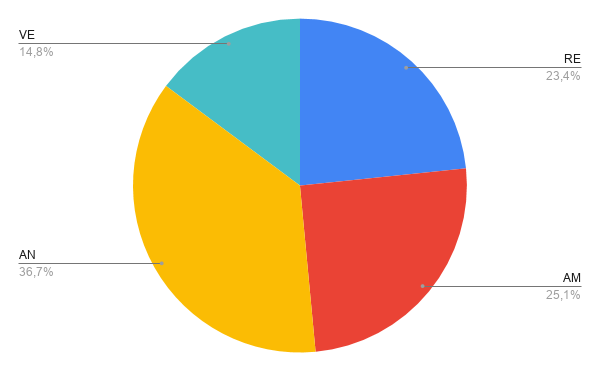
\includegraphics[width=0.8\linewidth]{../immagini/pdp/torta_analisi.png}
		\caption{Grafico a torta della ripartizione per ruolo delle ore nel periodo di Analisi}
	\end{center}
\end{figure}
\clearpage
\section{Fase di Consolidamento dei requisiti}\label{PreventivoFaseDiConsolidamentoDeiRequisiti}

\subsection{Prospetto orario}\label{PreventivoFaseDiConsolidamentoDeiRequisitiProspettoOrario}
In questa fase la distribuzione oraria è la seguente:
\quad
\def\tabularxcolumn#1{m{#1}}
{\rowcolors{2}{RawSienna!90!RawSienna!20}{RawSienna!70!RawSienna!40}

	\begin{center}
		\renewcommand{\arraystretch}{1.4}
		\begin{tabularx}{\textwidth}{|X|c|c|c|c|c|c|c|}
			\hline
			\rowcolor{airforceblue}
			\textbf{Nominativo} & \textbf{Re} & \textbf{Am} & \textbf{An} & \textbf{Pt} & \textbf{Pr} & \textbf{Ve} & \textbf{Totale ore}\\
			\hline
			\textit{Andrea Dorigo} & 0 & 2 & 0 & 0 & 0 & 2 & 4\\
			\hline
			\textit{Margherita Mitillo} & 0 & 2 & 1 & 0 & 0 & 1 & 4\\
			\hline
			\textit{Igli Mezini} & 1 & 1 & 0 & 0 & 0 & 2 & 4\\
			\hline
			\textit{Andrea Cecchin} & 1 & 0 & 2 & 0 & 0 & 1 & 4\\
			\hline
			\textit{Emma Roveroni} & 1 & 1 & 0 & 0 & 0 & 2 & 4\\
			\hline
			\textit{Alfredo Graziano} & 1 & 2 & 1 & 0 & 0 & 0 & 4\\
			\hline
			\textit{Mattia Cocco} & 1 & 0 & 1 & 0 & 0 & 2 & 4\\
			\hline
			Totale ore ruolo & 4 & 8 & 4 & 0 & 0 & 8 & 24\\
			\hline
		\end{tabularx}
	\captionof{table}{\textbf{distribuzione delle ore durante il Consolidamento dei requisiti}}
	\end{center}
Il seguente istogramma riassume i dati ottenuti:
\begin{figure}[!ht]
	\begin{center}
		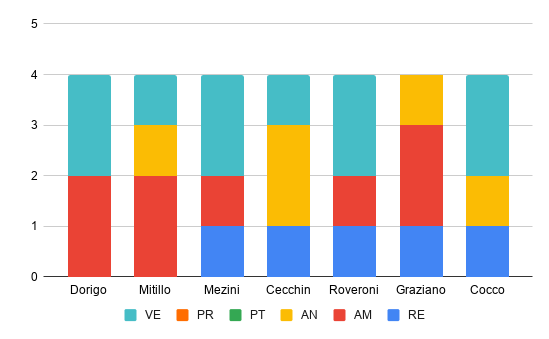
\includegraphics[width=0.7\linewidth]{../immagini/pdp/istogramma_consolidamento_requisiti.png}
		\caption{Istogramma della ripartizione oraria durante il Consolidamento dei requisiti
}
	\end{center}
\end{figure}

\subsection{Prospetto economico}\label{PreventivoFaseDiConsolidamentoDeiRequisitiProspettoEconomico}
\quad
\def\tabularxcolumn#1{m{#1}}
{\rowcolors{2}{RawSienna!90!RawSienna!20}{RawSienna!70!RawSienna!40}
	\begin{center}
		\renewcommand{\arraystretch}{1.4}
		\begin{tabularx}{7cm}{|X|c|c|}
			\hline
			\rowcolor{airforceblue}
			\textbf{Ruolo} & \textbf{Ore} & \textbf{Costo}\\
			\hline
			Responsabile & 4 & 120\euro\\
			\hline
			Amministratore & 8 & 160\euro\\
			\hline
			Analista & 4 & 100\euro\\
			\hline
			Progettista & 0 & 0\euro\\
			\hline
			Programmatore & 0 & 0\euro\\
			\hline
			Verificatore & 8 & 120\euro\\
			\hline
			Totale & 24 & 500\euro\\
			\hline
		\end{tabularx}
	\captionof{table}{\textbf{Prospetto dei costi per ruolo nel periodo di Consolidamento dei requisiti}}
	\end{center}
Il seguente grafico a torta riassume i dati ottenuti:
\begin{figure}[!ht]
	\begin{center}
		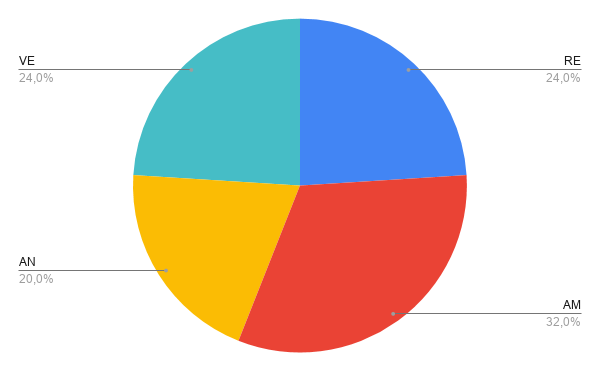
\includegraphics[width=0.8\linewidth]{../immagini/pdp/torta_consolidamento_requisiti.png}
		\caption{Grafico a torta della ripartizione per ruolo delle ore durante il periodo di Consolidamento dei requisiti}
	\end{center}
\end{figure}

\section{Fase di Progettazione architetturale}\label{PreventivoFaseDiProgettazioneArchitetturale}

\subsection{Prospetto orario}\label{PreventivoFaseDiProgettazioneArchitetturaleProspettoOrario}
In questa fase la distribuzione oraria è la seguente:
\quad
\def\tabularxcolumn#1{m{#1}}
{\rowcolors{2}{RawSienna!90!RawSienna!20}{RawSienna!70!RawSienna!40}

	\begin{center}
		\renewcommand{\arraystretch}{1.4}
		\begin{tabularx}{\textwidth}{|X|c|c|c|c|c|c|c|}
			\hline
			\rowcolor{airforceblue}
			\textbf{Nominativo} & \textbf{Re} & \textbf{Am} & \textbf{An} & \textbf{Pt} & \textbf{Pr} & \textbf{Ve} & \textbf{Totale ore}\\
			\hline
			\textit{Andrea Dorigo} & 5 & 3 & 2 & 16 & 4 & 5 & 35\\
			\hline
			\textit{Margherita Mitillo} & 5 & 7 & 2 & 12 & 0 & 9 & 35\\
			\hline
			\textit{Igli Mezini} & 4 & 2 & 8 & 8 & 3 & 10 & 35\\
			\hline
			\textit{Andrea Cecchin} & 7 & 5 & 4 & 10 & 2 & 7 & 35\\
			\hline
			\textit{Emma Roveroni} & 1 & 7 & 4 & 14 & 0 & 9 & 35\\
			\hline
			\textit{Alfredo Graziano} & 2 & 2 & 9 & 15 & 2 & 5 & 35\\
			\hline
			\textit{Mattia Cocco} & 6 & 2 & 6 & 11 & 1 & 9 & 35\\
			\hline
			Totale ore ruolo & 24 & 26 & 29 & 86 & 12 & 54 & 231\\
			\hline
		\end{tabularx}
	\captionof{table}{\textbf{distribuzione delle ore durante la Progettazione architetturale}}
	\end{center}

Il seguente istogramma riassume i dati ottenuti:
\begin{figure}[!h]
	\begin{center}
		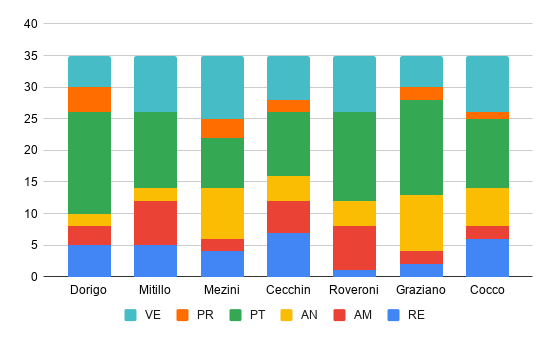
\includegraphics[width=0.7\linewidth]{../immagini/pdp/istogramma_progettazione_architetturale.png}
		\caption{Istogramma della ripartizione oraria durante la Progettazione architetturale}
	\end{center}
\end{figure}

\subsection{Prospetto economico}\label{PreventivoFaseDiProgettazioneArchitetturaleProspettoEconomico}
\quad
\def\tabularxcolumn#1{m{#1}}
{\rowcolors{2}{RawSienna!90!RawSienna!20}{RawSienna!70!RawSienna!40}
	\begin{center}
		\renewcommand{\arraystretch}{1.4}
		\begin{tabularx}{7cm}{|X|c|c|}
			\hline
			\rowcolor{airforceblue}
			\textbf{Ruolo} & \textbf{Ore} & \textbf{Costo}\\
			\hline
			Responsabile & 24 & 720\euro\\
			\hline
			Amministratore & 26 & 520\euro\\
			\hline
			Analista & 29 & 725\euro\\
			\hline
			Progettista & 86 & 1892\euro\\
			\hline
			Programmatore & 12 & 180\euro\\
			\hline
			Verificatore & 54 & 810\euro\\
			\hline
			Totale & 231 & 4847\euro\\
			\hline
		\end{tabularx}
	\captionof{table}{\textbf{Prospetto dei costi per ruolo nel periodo di Progettazione architetturale}}
	\end{center}

Il seguente grafico a torta riassume i dati ottenuti:
\begin{figure}[!ht]
	\begin{center}
		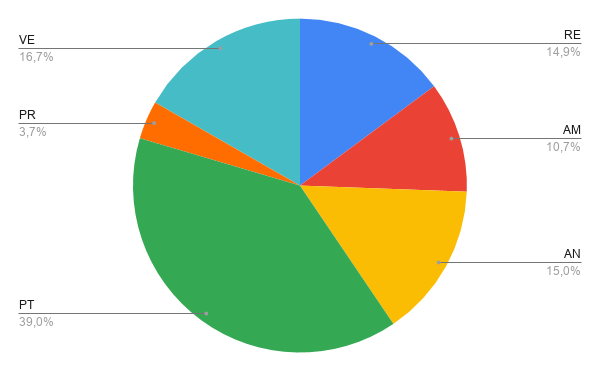
\includegraphics[width=0.8\linewidth]{../immagini/pdp/torta_progettazione_architetturale.png}
		\caption{Grafico a torta della ripartizione per ruolo delle ore nel periodo di Progettazione architetturale}
	\end{center}
\end{figure}

\section{Fase di Progettazione di dettaglio e codifica}\label{PreventivoFaseDiProgettazioneDiDettaglioECodifica}

\subsection{Prospetto orario}\label{PreventivoFaseDiProgettazioneDiDettaglioECodificaProspettoOrario}
In questa fase la distribuzione oraria è la seguente:
\quad
\def\tabularxcolumn#1{m{#1}}
{\rowcolors{2}{RawSienna!90!RawSienna!20}{RawSienna!70!RawSienna!40}

	\begin{center}
		\renewcommand{\arraystretch}{1.4}
		\begin{tabularx}{\textwidth}{|X|c|c|c|c|c|c|c|}
			\hline
			\rowcolor{airforceblue}
			\textbf{Nominativo} & \textbf{Re} & \textbf{Am} & \textbf{An} & \textbf{Pt} & \textbf{Pr} & \textbf{Ve} & \textbf{Totale ore}\\
			\hline
			\textit{Andrea Dorigo} & 8 & 7 & 4 & 9 & 8 & 9 & 45\\
			\hline
			\textit{Margherita Mitillo} & 4 & 6 & 5 & 8 & 9 & 13 & 45\\
			\hline
			\textit{Igli Mezini} & 3 & 8 & 2 & 10 & 11 & 11 & 45\\
			\hline
			\textit{Andrea Cecchin} & 4 & 3 & 2 & 11 & 14 & 11 & 45\\
			\hline
			\textit{Emma Roveroni} & 7 & 4 & 3 & 11 & 8 & 12 & 45\\
			\hline
			\textit{Alfredo Graziano} & 5 & 6 & 3 & 10 & 11 & 10 & 45\\
			\hline
			\textit{Mattia Cocco} & 4 & 4 & 7 & 10 & 10 & 10 & 45\\
			\hline
			Totale ore ruolo & 31 & 34 & 19 & 69 & 61 & 66 & 280\\
			\hline
		\end{tabularx}
	\captionof{table}{\textbf{Distribuzione delle ore durante la Progettazione di dettaglio e codifica}}
	\end{center}
Il seguente istogramma riassume i dati ottenuti:
\begin{figure}[!h]
	\begin{center}
		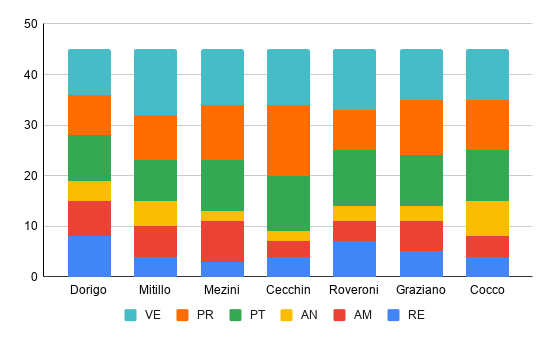
\includegraphics[width=0.7\linewidth]{../immagini/pdp/istogramma_progettazione_dettaglio.png}
		\caption{Istogramma della ripartizione oraria durante la Progettazione di
			dettaglio e codifica}
	\end{center}
\end{figure}
\clearpage
\subsection{Prospetto economico}\label{PreventivoFaseDiProgettazioneDiDettaglioECodificaProspettoEconomico}
\quad
\def\tabularxcolumn#1{m{#1}}
{\rowcolors{2}{RawSienna!90!RawSienna!20}{RawSienna!70!RawSienna!40}
	\begin{center}
		\renewcommand{\arraystretch}{1.4}
		\begin{tabularx}{7cm}{|X|c|c|}
			\hline
			\rowcolor{airforceblue}
			\textbf{Ruolo} & \textbf{Ore} & \textbf{Costo}\\
			\hline
			Responsabile & 31 & 930\euro\\
			\hline
			Amministratore & 34 & 680\euro\\
			\hline
			Analista & 19 & 475\euro\\
			\hline
			Progettista & 69 & 1518\euro\\
			\hline
			Programmatore & 61 & 915\euro\\
			\hline
			Verificatore & 66 & 990\euro\\
			\hline
			Totale & 280 & 5508\euro\\
			\hline
		\end{tabularx}
	\captionof{table}{\textbf{Prospetto dei costi per ruolo nel periodo di Progettazione di dettaglio e codifica}}
	\end{center}

Il seguente grafico a torta riassume i dati ottenuti:
\begin{figure}[!ht]
	\begin{center}
		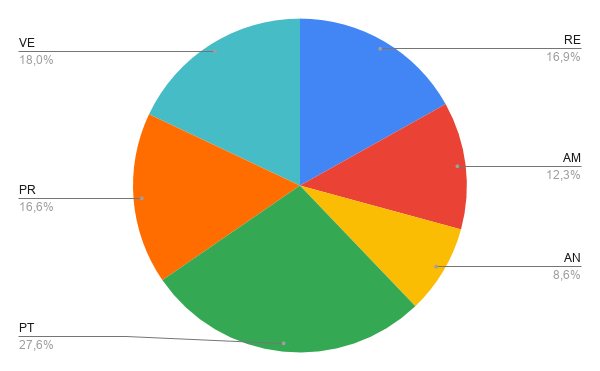
\includegraphics[width=0.8\linewidth]{../immagini/pdp/torta_progettazione_dettaglio.png}
		\caption{Grafico a torta della ripartizione per ruolo delle ore nel periodo di Progettazione
			di dettaglio e codifica}
	\end{center}
\end{figure}

\section{Fase di Progettazione di Validazione e collaudo}\label{PreventivoFaseDiProgettazionediValidazioneECollaudo}

\subsection{Prospetto orario}\label{PreventivoPreventivoFaseDiProgettazionediValidazioneECollaudoProspettoOrario}
In questa fase la distribuzione oraria è la seguente:
\quad
\def\tabularxcolumn#1{m{#1}}
{\rowcolors{2}{RawSienna!90!RawSienna!20}{RawSienna!70!RawSienna!40}

	\begin{center}
		\renewcommand{\arraystretch}{1.4}
		\begin{tabularx}{\textwidth}{|X|c|c|c|c|c|c|c|}
			\hline
			\rowcolor{airforceblue}
			\textbf{Nominativo} & \textbf{Re} & \textbf{Am} & \textbf{An} & \textbf{Pt} & \textbf{Pr} & \textbf{Ve} & \textbf{Totale ore}\\
			\hline
			\textit{Andrea Dorigo} & 6 & 6 & 0 & 0 & 6 & 7 & 25\\
			\hline
			\textit{Margherita Mitillo} & 3 & 7 & 0 & 0 & 9 & 6 & 25\\
			\hline
			\textit{Igli Mezini} & 4 & 2 & 0 & 0 & 10 & 9 & 25\\
			\hline
			\textit{Andrea Cecchin} & 2 & 1 & 0 & 0 & 12 & 10 & 25\\
			\hline
			\textit{Emma Roveroni} & 2 & 3 & 0 & 0 & 10 & 10 & 25\\
			\hline
			\textit{Alfredo Graziano} & 3 & 3 & 0 & 0 & 9 & 10 & 25\\
			\hline
			\textit{Mattia Cocco} & 1 & 6 & 0 & 0 & 10 & 8 & 25\\
			\hline
			Totale ore ruolo & 21 & 28 & 0 & 0 & 66 & 60 & 175\\
			\hline
		\end{tabularx}
	\captionof{table}{\textbf{distribuzione delle ore durante la Validazione e collaudo}}
	\end{center}
Il seguente istogramma riassume i dati ottenuti:
\begin{figure}[!ht]
	\begin{center}
		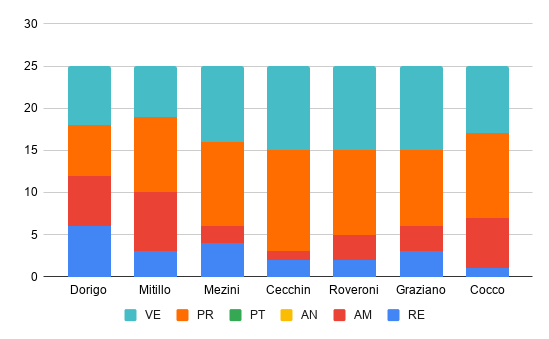
\includegraphics[width=0.7\linewidth]{../immagini/pdp/istogramma_validazione.png}
		\caption{Istogramma della ripartizione oraria durante la Validazione e
			collaudo}
	\end{center}
\end{figure}
\clearpage
\subsection{Prospetto economico}\label{PreventivoPreventivoFaseDiProgettazionediValidazioneECollaudoProspettoEconomico}
\quad
\def\tabularxcolumn#1{m{#1}}
{\rowcolors{2}{RawSienna!90!RawSienna!20}{RawSienna!70!RawSienna!40}
	\begin{center}
		\renewcommand{\arraystretch}{1.4}
		\begin{tabularx}{7cm}{|X|c|c|}
			\hline
			\rowcolor{airforceblue}
			\textbf{Ruolo} & \textbf{Ore} & \textbf{Costo}\\
			\hline
			Responsabile & 21 & 630\euro\\
			\hline
			Amministratore & 28 & 560\euro\\
			\hline
			Analista & 0 & 0\euro\\
			\hline
			Progettista & 0 & 0\euro\\
			\hline
			Programmatore & 66 & 990\euro\\
			\hline
			Verificatore & 60 & 900\euro\\
			\hline
			Totale & 175 & 3080\euro\\
			\hline
		\end{tabularx}
	\captionof{table}{\textbf{Prospetto dei costi per ruolo nel periodo di Progettazione di Validazione e collaudo}}
	\end{center}

Il seguente grafico a torta riassume i dati ottenuti:
\begin{figure}[!ht]
	\begin{center}
		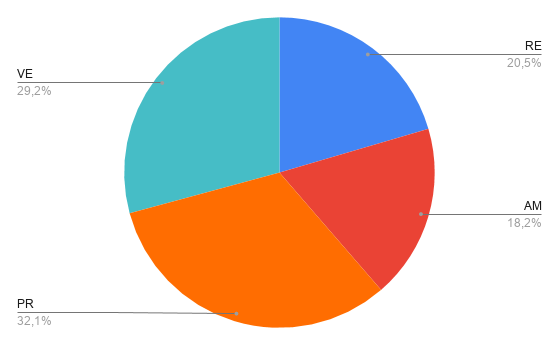
\includegraphics[width=0.8\linewidth]{../immagini/pdp/torta_validazione.png}
		\caption{Grafico a torta della ripartizione per ruolo delle ore nel periodo di Validazione e Collaudo}
	\end{center}
\end{figure}

\section{Riepilogo}\label{PreventivoRiepilogo}

\subsection{Ore totali}\label{PreventivoRiepilogoOreTotali}

\subsubsection{Suddivisione lavoro}\label{PreventivoRiepilogoOreTotaliSuddivisioneDelLavoro}
Nella seguente tabella vengono riportate il totale delle ore del progetto, sono presenti sia le ore di investimento, sia quelle rendicontate a carico del committente$_G$.
\quad
\def\tabularxcolumn#1{m{#1}}
{\rowcolors{2}{RawSienna!90!RawSienna!20}{RawSienna!70!RawSienna!40}

	\begin{center}
		\renewcommand{\arraystretch}{1.4}
		\begin{tabularx}{\textwidth}{|X|c|c|c|c|c|c|c|}
			\hline
			\rowcolor{airforceblue}
			\textbf{Nominativo} & \textbf{Re} & \textbf{Am} & \textbf{An} & \textbf{Pt} & \textbf{Pr} & \textbf{Ve} & \textbf{Totale ore}\\
			\hline
			\textit{Andrea Dorigo} & 29 & 25 & 9 & 25 & 18 & 28 & 134\\
			\hline
			\textit{Margherita Mitillo} & 20 & 25 & 21 & 20 & 18 & 30 & 134\\
			\hline
			\textit{Igli Mezini} & 15 & 19 & 18 & 18 & 24 & 40 & 134\\
			\hline
			\textit{Andrea Cecchin} & 19 & 18 & 17 & 21 & 28 & 31 & 134\\
			\hline
			\textit{Emma Roveroni} & 11 & 22 & 14 & 25 & 18 & 44 & 134\\
			\hline
			\textit{Alfredo Graziano} & 11 & 23 & 22 & 25 & 22 & 31 & 134\\
			\hline
			\textit{Mattia Cocco} & 13 & 21 & 22 & 21 & 21 & 36 & 134\\
			\hline
		\end{tabularx}
	\captionof{table}{\textbf{Distribuzione delle ore totali di investimento e rendicontate}}
	\end{center}

Il seguente istogramma riassume i dati ottenuti:
\begin{figure}[!h]
	\begin{center}
		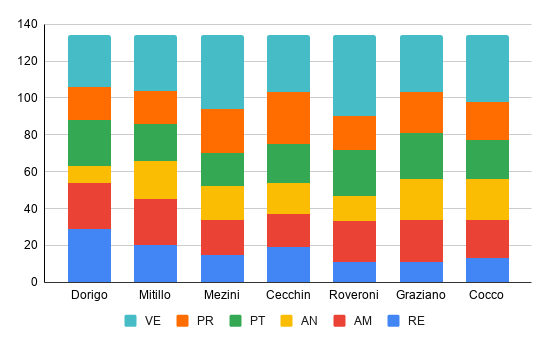
\includegraphics[width=0.65\linewidth]{../immagini/pdp/istogramma_suddivisione_lavoro.png}
		\caption{Istogramma della ripartizione oraria totali di investimento e rendicontate}
	\end{center}
\end{figure}

\subsubsection{Prospetto economico}\label{PreventivoRiepilogoOreTotaliProspettoEconomico}
I costi da affrontare per ogni ruolo sono:
\quad
\def\tabularxcolumn#1{m{#1}}
{\rowcolors{2}{RawSienna!90!RawSienna!20}{RawSienna!70!RawSienna!40}
	\begin{center}
		\renewcommand{\arraystretch}{1.4}
		\begin{tabularx}{7cm}{|X|c|c|}
			\hline
			\rowcolor{airforceblue}
			\textbf{Ruolo} & \textbf{Ore} & \textbf{Costo}\\
			\hline
			Responsabile & 118 & 3540\euro\\
			\hline
			Amministratore & 153 & 3060\euro\\
			\hline
			Analista & 123 & 3075\euro\\
			\hline
			Progettista & 155 & 3410\euro\\
			\hline
			Programmatore & 149 & 2235\\
			\hline
			Verificatore & 240 & 3600\\
			\hline
			Totale & 938 & 18920\euro\\
			\hline
		\end{tabularx}
	\captionof{table}{\textbf{Prospetto dei costi totali delle ore totali di investimento e rendicontate}}
	\end{center}

Il seguente grafico a torta riassume i dati ottenuti:
\begin{figure}[!ht]
	\begin{center}
		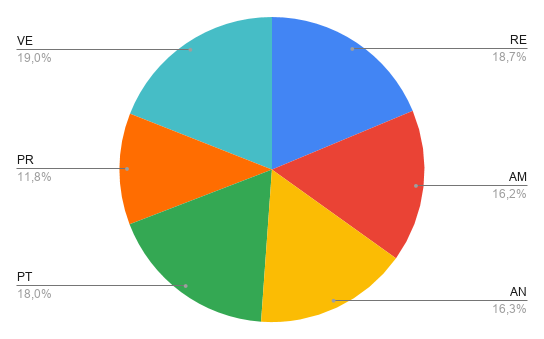
\includegraphics[width=0.8\linewidth]{../immagini/pdp/torta_suddvisione_lavoro.png}
		\caption{Grafico a torta della ripartizione per ruolo delle ore totali di investimento e
			rendicontate}
	\end{center}
\end{figure}

\subsection{Ore rendicontate}\label{PreventivoRiepilogoOreRendicontate}

\subsubsection{Suddivisione lavoro}\label{PreventivoRiepilogoOreRendicontateSuddivisioneLavoro}
Le ore rendicontate sono riportate nella seguente tabella:
\quad
\def\tabularxcolumn#1{m{#1}}
{\rowcolors{2}{RawSienna!90!RawSienna!20}{RawSienna!70!RawSienna!40}

	\begin{center}
		\renewcommand{\arraystretch}{1.4}
		\begin{tabularx}{\textwidth}{|X|c|c|c|c|c|c|c|}
			\hline
			\rowcolor{airforceblue}
			\textbf{Nominativo} & \textbf{Re} & \textbf{Am} & \textbf{An} & \textbf{Pt} & \textbf{Pr} & \textbf{Ve} & \textbf{Totale ore}\\
			\hline
			\textit{Andrea Dorigo} & 19 & 16 & 6 & 25 & 18 & 21 & 105\\
			\hline
			\textit{Margherita Mitillo} & 12 & 20 & 7 & 20 & 18 & 28 & 105\\
			\hline
			\textit{Igli Mezini} & 11 & 12 & 10 & 18 & 24 & 30 & 105\\
			\hline
			\textit{Andrea Cecchin} & 13 & 9 & 6 & 21 & 28 & 28 & 105\\
			\hline
			\textit{Emma Roveroni} & 10 & 14 & 7 & 25 & 18 & 31 & 105\\
			\hline
			\textit{Alfredo Graziano} & 10 & 11 & 12 & 25 & 22 & 25 & 105\\
			\hline
			\textit{Mattia Cocco} & 11 & 12 & 13 & 21 & 21 & 27 & 105\\
			\hline
		\end{tabularx}
	\captionof{table}{\textbf{Distribuzione delle ore rendicontate}}
	\end{center}
Il seguente istogramma riassume i dati ottenuti:
\begin{figure}[!ht]
	\begin{center}
		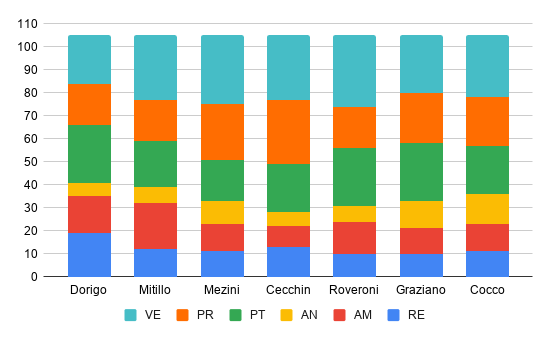
\includegraphics[width=0.8\linewidth]{../immagini/pdp/istogramma_rendicontate.png}
		\caption{Istogramma della ripartizione oraria rendicontate}
	\end{center}
\end{figure}

\subsubsection{Prospetto economico}\label{PreventivoRiepilogoOreRendicontateProspettoEconomico}
Il totale rendicontato dei costi da affrontare per ogni ruolo è il seguenti:
\quad
\def\tabularxcolumn#1{m{#1}}
{\rowcolors{2}{RawSienna!90!RawSienna!20}{RawSienna!70!RawSienna!40}
	\begin{center}
		\renewcommand{\arraystretch}{1.4}
		\begin{tabularx}{7cm}{|X|c|c|}
			\hline
			\rowcolor{airforceblue}
			\textbf{Ruolo} & \textbf{Ore} & \textbf{Costo}\\
			\hline
			Responsabile & 86 & 2580\euro\\
			\hline
			Amministratore & 94 & 1880\euro\\
			\hline
			Analista & 61 & 1525\euro\\
			\hline
			Progettista & 155 & 3410\euro\\
			\hline
			Programmatore & 149 & 2235\euro\\
			\hline
			Verificatore & 190 & 2850\euro\\
			\hline
			Totale & 735 & 14480\euro\\
			\hline
		\end{tabularx}
	\captionof{table}{\textbf{Prospetto dei costi totali delle ore rendicontate}}
	\end{center}
Il seguente grafico a torta riassume i dati ottenuti:
\begin{figure}[!ht]
	\begin{center}
		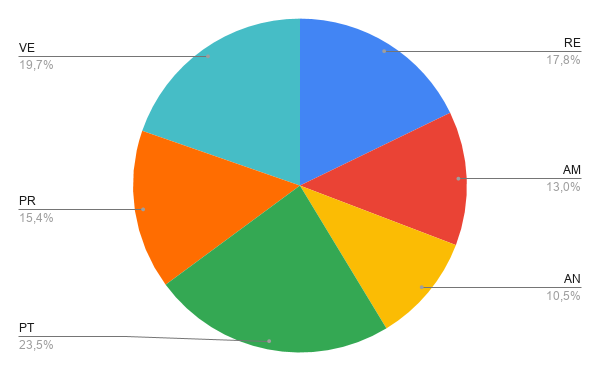
\includegraphics[width=0.8\linewidth]{../immagini/pdp/torta_rendicontate.png}
		\caption{Grafico a torta della ripartizione per ruolo delle ore rendicontate}
	\end{center}
\end{figure}
\subsection{Conclusioni}\label{PreventivoRiepilogoConclusioni}
Il costo totale del progetto considerando solamente le ore rendicontate è: 14480\euro.
